\documentclass{article}
\usepackage[T1]{fontenc}
\usepackage[utf8]{inputenc}
\usepackage[margin=1in]{geometry}
\usepackage{fancyhdr} 
\usepackage{listings}
\usepackage{xcolor}

\definecolor{keywordcolor}{rgb}{0.4, 0.7, 1.0} % Light blue for keywords
\definecolor{ndkeywordcolor}{rgb}{0.8, 0.5, 0.0} % Orange for non-default keywords
\definecolor{stringcolor}{rgb}{0.8, 0.2, 0.2} % Red for strings
\definecolor{commentcolor}{rgb}{0.6, 0.6, 0.6} % Gray for comments
\definecolor{bracecolor}{rgb}{0.6, 0.6, 1.0} % Custom color for braces

\lstdefinelanguage{JavaScript}{
  keywords={break, case, catch, continue, debugger, default, delete, do, else, finally, for, function, if, in, instanceof, new, return, switch, this, throw, try, typeof, var, void, while, with},
  keywordstyle=\color{keywordcolor}\bfseries,
  ndkeywords={class, export, boolean, throw, implements, import, this},
  ndkeywordstyle=\color{ndkeywordcolor}\bfseries,
  identifierstyle=\color{black},
  sensitive=false,
  comment=[l]{//},
  morecomment=[s]{/*}{*/},
  commentstyle=\color{commentcolor}\itshape,
  stringstyle=\color{stringcolor}\ttfamily,
  morestring=[b]',
  morestring=[b]",
  literate={\{}{{\textcolor{bracecolor}{\{}}}1
           {\}}{{\textcolor{bracecolor}{\}}}}1
           {<}{{\textcolor{bracecolor}{<}}}1
           {>}{{\textcolor{bracecolor}{>}}}1,
}
\lstdefinelanguage{Python3}{
  keywords={False, async, class, finally, is, return, None, continue, for, lambda, try, True, def, from, nonlocal, while, and, del, global, not, with, as, elif, if, or, yield, assert, else, import, pass, break, except, in, raise},
  keywordstyle=\color{blue}\bfseries,
  ndkeywords={self},
  ndkeywordstyle=\color{darkgray}\bfseries,
  identifierstyle=\color{black},
  sensitive=true,
  comment=[l]{\#},
  morecomment=[s]{"""}{"""},
  commentstyle=\color{purple}\ttfamily,
  stringstyle=\color{red}\ttfamily,
  morestring=[b]',
  morestring=[b]",
  emph={print, len, range, int, str, float, list, dict, set, tuple},
  emphstyle={\color{teal}}
}
\usepackage[ruled,vlined]{algorithm2e}
\usepackage{amsthm}
\usepackage{amsfonts}
\usepackage{amssymb}
\usepackage{graphicx}
\usepackage[dvipsnames]{xcolor}
\usepackage{xy}
% \usepackage{url} % Commented out because hyperref provides similar functionality
\usepackage{parskip}
\usepackage{comment}
\usepackage{setspace}
\usepackage{enumerate}
\usepackage{multirow}
\usepackage{hyperref}
\usepackage{caption}
\usepackage{subcaption}
\usepackage{booktabs}
\usepackage{wrapfig}
\usepackage{times}

\captionsetup[figure]{font={small,it}}

\usepackage[backend=biber,style=numeric,sortcites,maxbibnames=99]{biblatex}
\addbibresource{references.bib}

\newcommand{\HRule}{\rule{\linewidth}{0.5mm}}
\newcommand{\Hrule}{\rule{\linewidth}{0.3mm}}
\newcommand{\classnum}{CS-GY 6313 B}

\makeatletter% since there's an at-sign (@) in the command name
\renewcommand{\@maketitle}{%
  \parindent=0pt% don't indent paragraphs in the title block
  \centering
  {\Large \bfseries\textsc{\@title}}
  \HRule\par%
  \textit{\@author \hfill \classnum}
  \par
}
\makeatother% resets the meaning of the at-sign (@)

\title{Assignment 3: Interactive Visualization} 
\author{Ivan Aristy — iae225}
% \classnum

\begin{document}
  \maketitle % prints the title block
  \thispagestyle{empty}
  % \vspace{-15pt}

\section{Interactive Visualization}
\label{sec:sec1}

Note 1: For the puposes of page limits,
I am treating code blocks as figures; 
hence, they should not be considered.

Note 2: The typesetting for the code blocks (lstdefinelanguage classes) 
was made with AI, since this is not at all core to the assignment,
I believe this usage is within the course guidelines.

\subsection{Question }
\label{subsec:subsec1}

\textbf{How has my champion's win rate changed over time? Is my champion still strong in the current meta?}

I want the user to easily see the win rate of their champion over time. 
Winrate is a key metric in League of Legends, as it is a good indicator of how strong a champion is in the current meta.
This would allow the user to see how their champion has been impacted in recent patches.

Winrate is not a direct representation of power, since some champions are harder to play than others.
Easy champions usually have high winrates, while hard champions have lower winrates.
Additionally, hyper-specific champions have really high winrates, since they are only played in specific situations.

Nevertheless, patterns in winrates can be indicative of power. For example, a 2\% growth in winrates
over a patch can be indicative of a very strong relating buff, while a 2\% decrease can be indicative of a strong relative nerf.
Additionally, a winrate that is consistently above 50\% can show that a champion has and is strong in the current meta.

\subsection{Data}
\label{subsec:subsec2}

\subsubsection{Data Source}
\label{subsubsec:Data Source}

Riot's Developer API is very hard to use. In my opinion, it is not well documented, and it is very hard to get the data you want.
Hence, I wll scrape some data off the internet to get the winrate of a champion over time.

Particularly I need:
\begin{enumerate}
  \item The winrate of a champions over time.
  \item The tier of the champion over time.
  \item Visual Assets of the champion.
\end{enumerate}

\subsubsection{Data Retreival} 
\label{subsubsec:Data Retreival}

To get winrate data, I will scrape \url{https://lolalytics.com/lol/tierlist/} for the winrate and tier of a champion over time.

After analyzing the beautiful soup output, the relevant information for a champion 
is contained in a div with the class \texttt{flex justify-around border border-[\#333333] p-2 text-center}.
For the next div, we will skip the explanation, but it uses a similar process to the code below.

\begin{figure}[ht] 
  \centering
  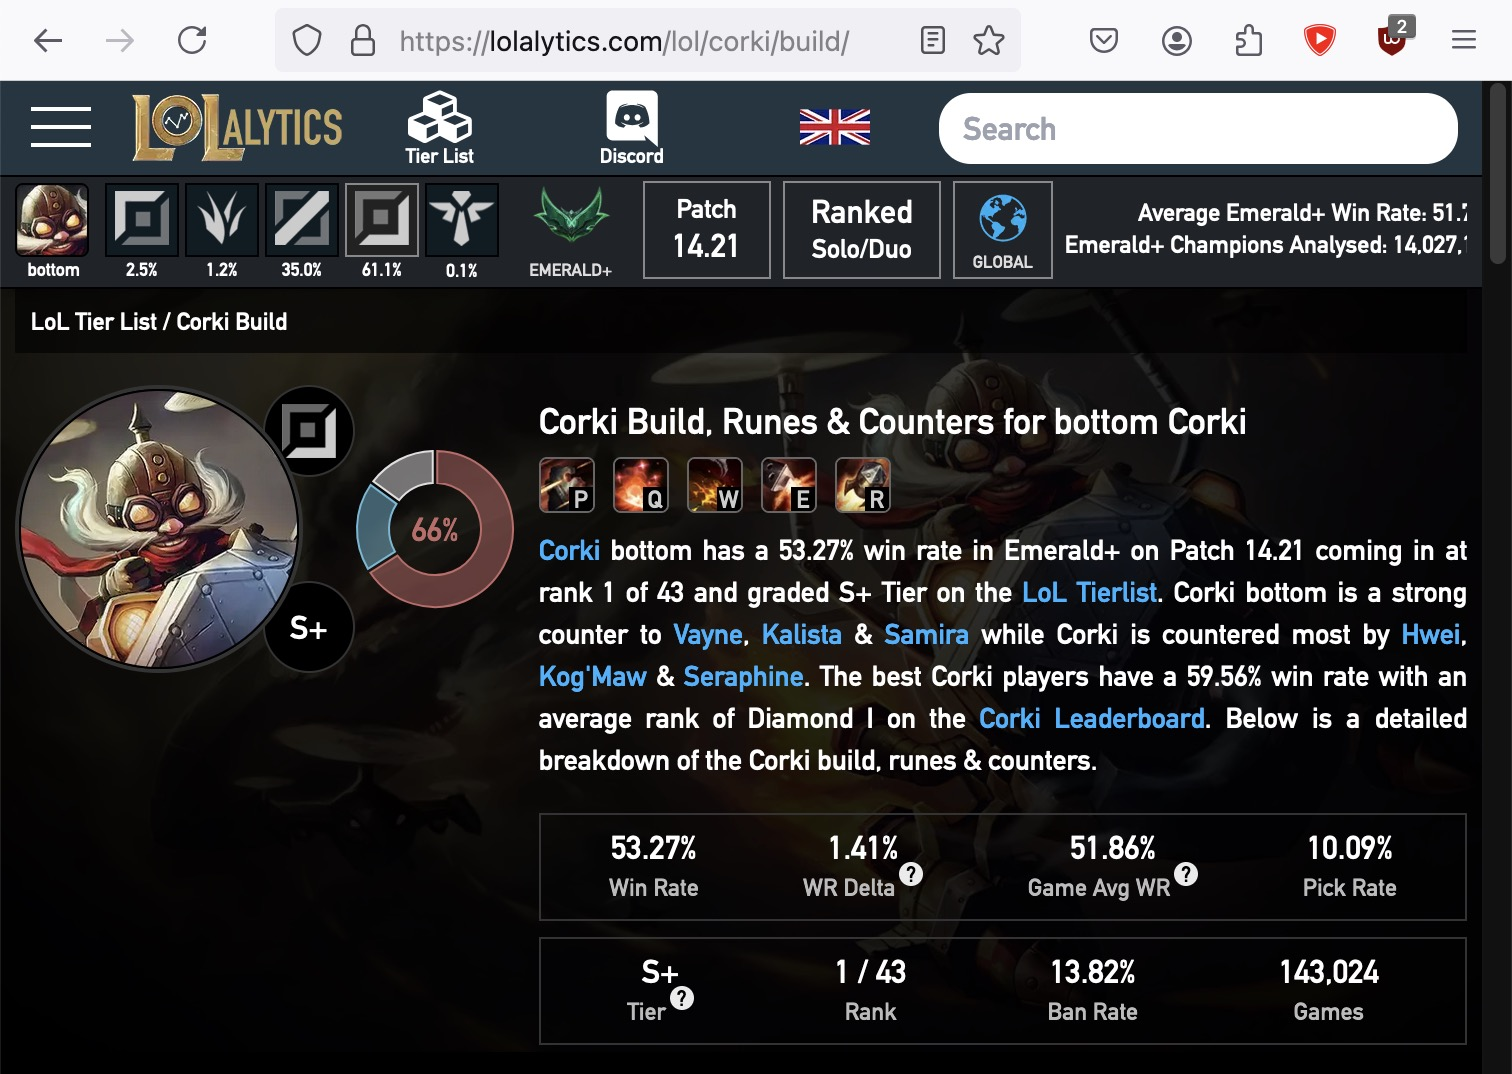
\includegraphics[width=0.75\textwidth]{figs/website.jpg}
  \caption{
      Corki's champion page.
  }
  \label{fig:fig1}
\end{figure}

\begin{lstlisting}[language=Javascript]
  container_div = soup.find('div', class_='flex justify-around 
  border border-[#333333] p-2 text-center')
  if container_div:
      # Find all the individual sections within this container
      sections = container_div.find_all('div', recursive=False)
      
      for section in sections:
          value_div = section.find('div', class_='mb-1 font-bold')
          if value_div:
              value = value_div.get_text(strip=True)
              row_1_data.append(value)
  print(row_1_data)
\end{lstlisting}

In \autoref{fig:fig1} the relevant data would be the eight values from "Win Rate"
to "Games". However, this information is only for one patch, so the backend
function will also receive a parameter to indicate the patch to scrape.

\subsubsection{Serving Backend Server} 
\label{subsubsec:Serving Backend Server}

We are using FastAPI to expose the data to the frontend. 
To accurately model the data, I created the following interface:

\begin{lstlisting}[language=Python3]
class ChampionInstance(BaseModel):
  name: str
  patch: float
  win_rate: float
  win_rate_delta: float
  modified_winrate: float
  pick_rate: float
  tier: str
  rank: int
  ban_rate: float
  games: int
\end{lstlisting}

and exposed the following function to the frontend:

\begin{lstlisting}[language=Python3]
@app.get("/test/{champion_name}&{patch_version}")
async def test(champion_name: str, patch_version: str):
  testChampion: ChampionInstance = 
    await api.get_champion_data(champion_name, patch_version)
  return testChampion
\end{lstlisting}

All the functions used were made asynchronous, since load times were a complaint 
I received from my peers while showing them the assignment. 

The benefit of using live data is that, whenever a new patch is released, the user can see how their champion has been impacted by the patch.
Additionally, for the current patch, changes in data are reflected in real time.

% \begin{figure}[ht] % Change the position of your figure https://www.overleaf.com/learn/latex/Positioning_images_and_tables
%   \centering
%   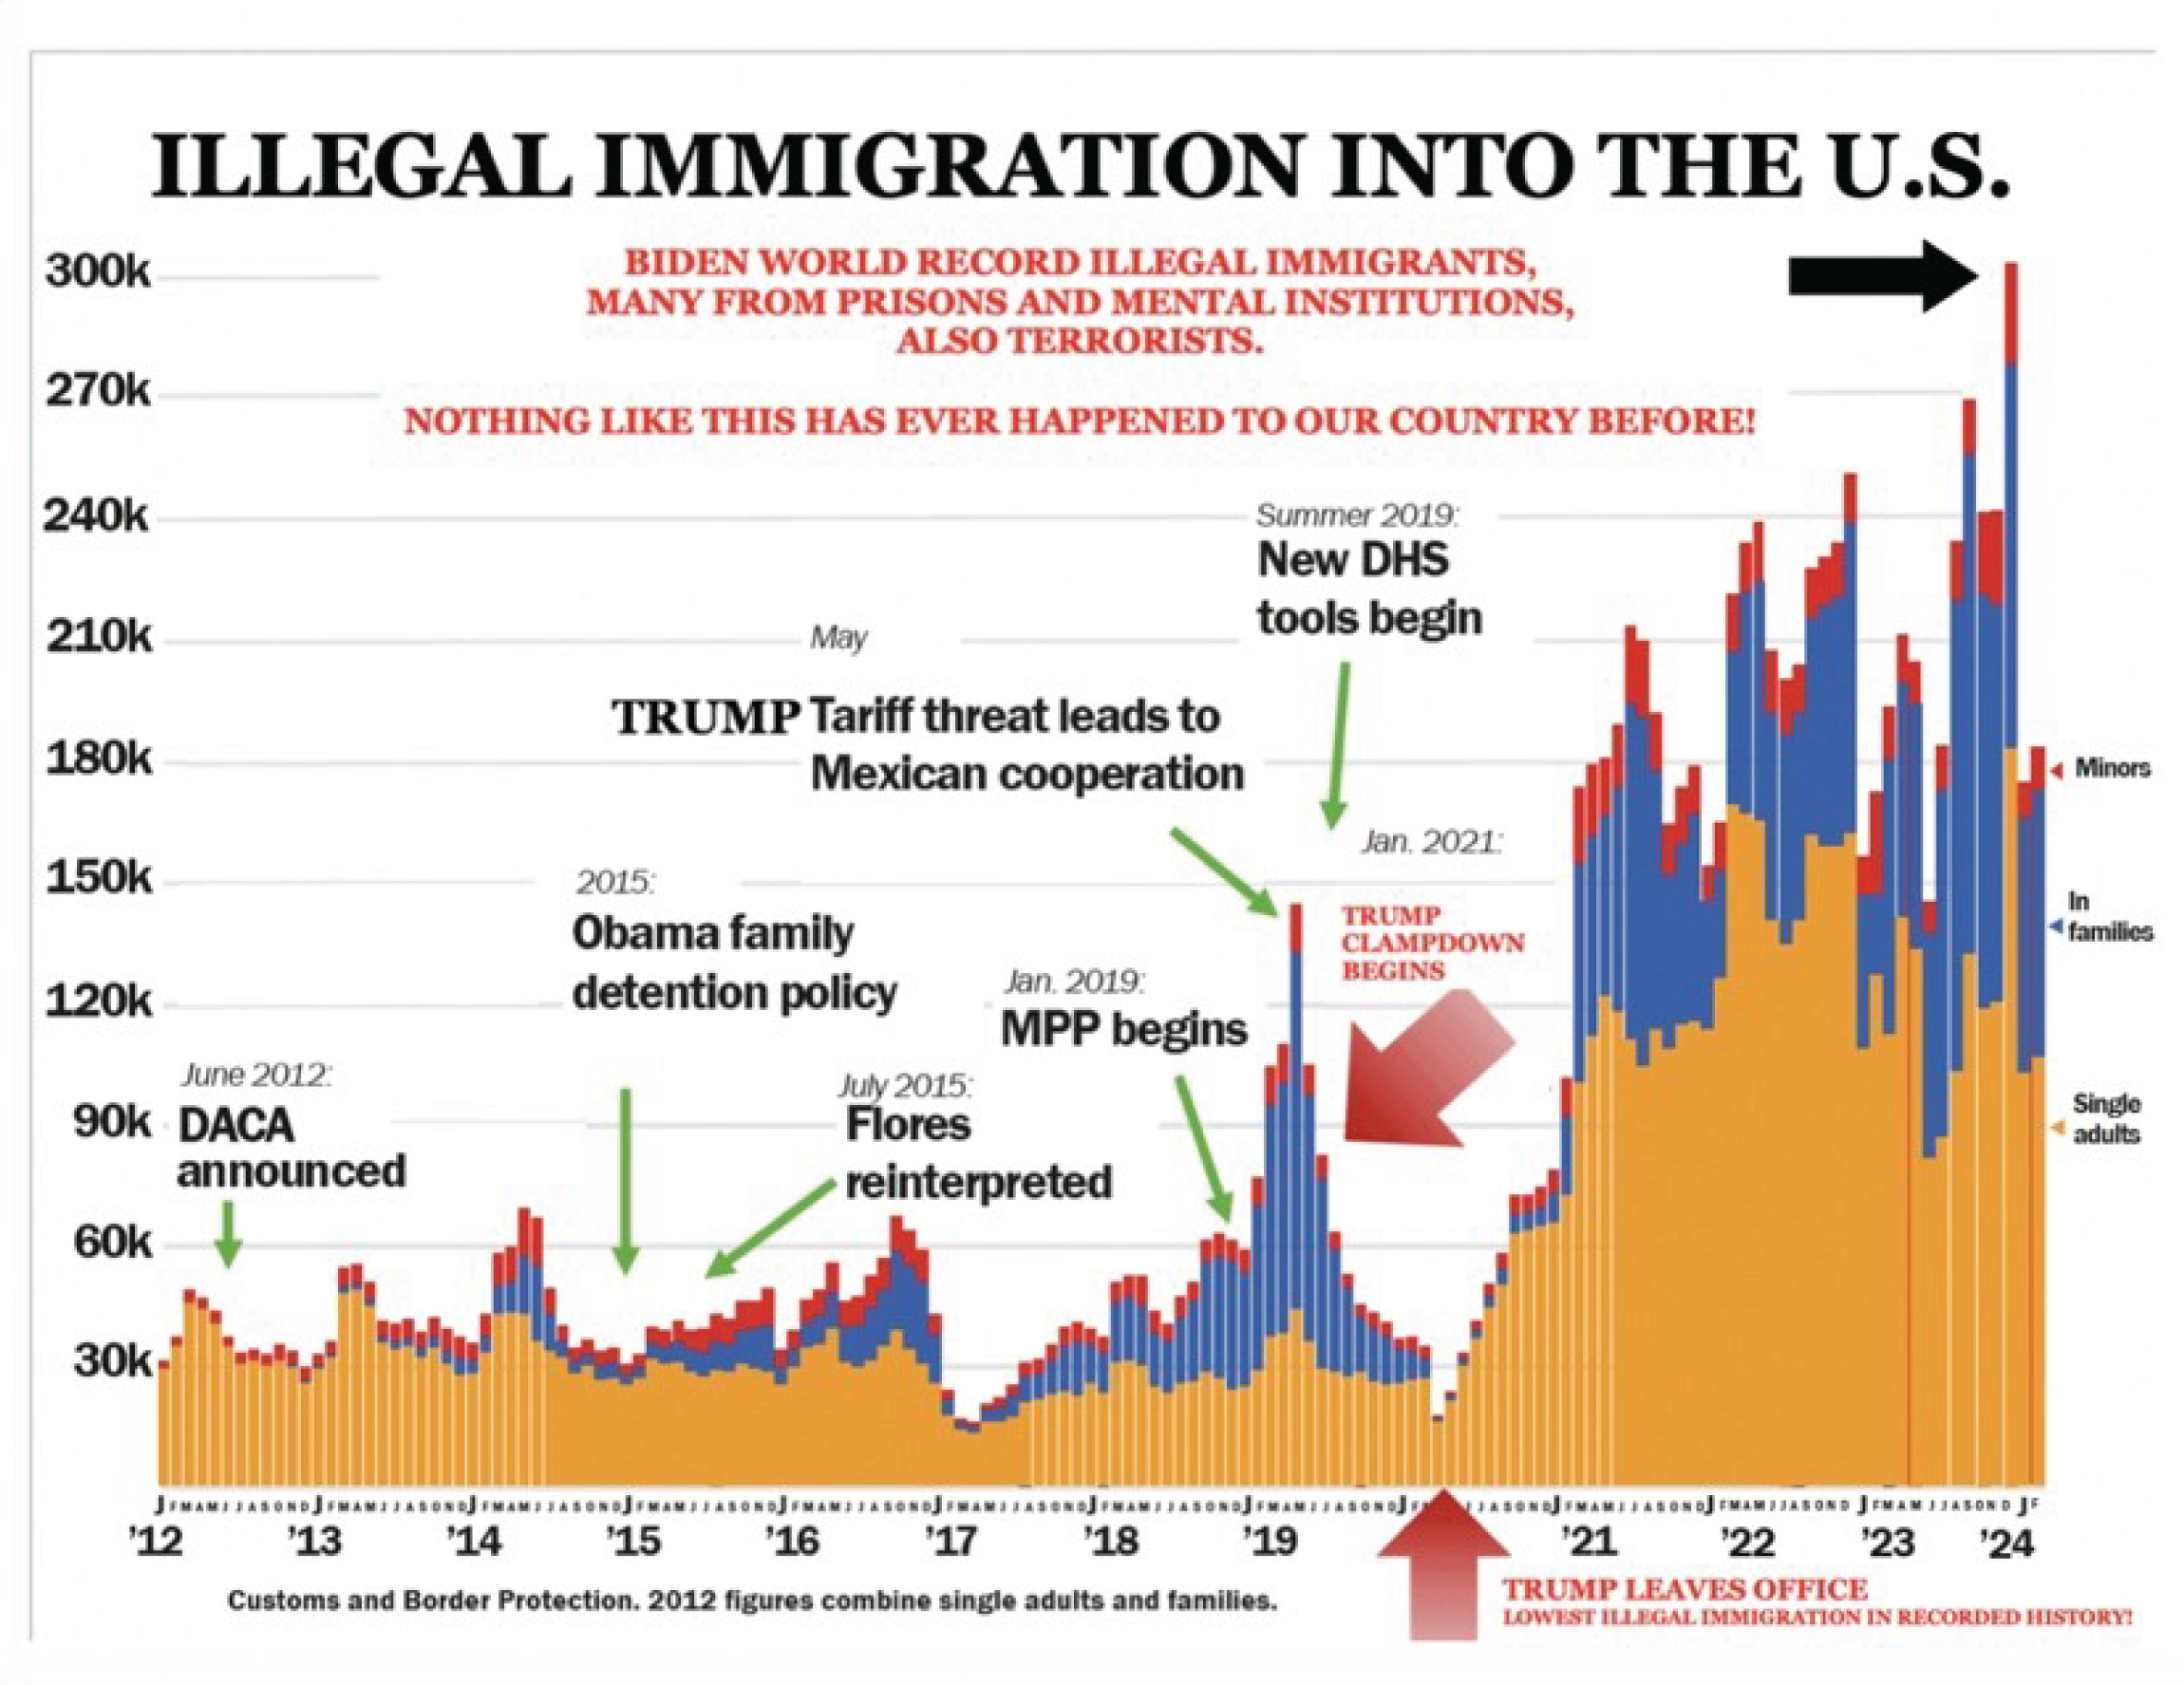
\includegraphics[width=0.75\textwidth]{figs/Trump Chart.png}
%   \caption{
%       Trump's Illegal Immigration Chart
%   }
%   \label{fig:fig1}
% \end{figure}

\subsection{Visualization}
\label{subsec:Visualization}

\subsubsection{Frontend Setup}
\label{subsubsec:Frontend}

The frontend is a simple React application that uses the 
\texttt{D3} library to create the chart, and react hooks to update 
and keep track of state (dynamic reloading of data depending on user
selected parameters).

For the main App component, we define a useEffect hook that will achieve
multiple "Quality of Life" improvements for the user:
\begin{itemize}
  \item Updating the chart whenever the user selects a new champion, metric, or patch range.
  \item Displaying a loading spinner while the data is being fetched.
  \item Asynchronous fetching of data to speed up the loading process.
  \item Invalidate erroneous data but keep plotting the chart.
\end{itemize}

\begin{lstlisting}[language=Javascript]
useEffect(() => {
    async function fetchData() {
      setLoading(true);

      const patchRange = patches.slice(
        patches.indexOf(startPatch),
        patches.indexOf(endPatch) + 1
      );

      try {
        const results = await Promise.all(
          patchRange.map(async (patch) => {
            const response = await fetch(
              `http://127.0.0.1:8000/test/${selectedChampion}&${patch}`
            );
            if (!response.ok)
              throw new Error(`Failed to fetch data for patch ${patch}`);

            const result = await response.json();
            return { patch, value: result[selectedMetric] };
          })
        );

        setData(results);
      } catch (error) {
        console.error("An error occurred while fetching data:", error);
      } finally {
        setLoading(false);
      }
    }

    setData(null);
    fetchData();
  }, [selectedChampion, selectedMetric, startPatch, endPatch]);
\end{lstlisting}

\subsubsection{Interactivity Logic}
\label{subsubsec:Interactivity Logic}

To allow for interactivity, we create a few drop down labels that allow the user
to select the data that they want to plot. For example, here is the code
for the "Champion" Label:

\begin{lstlisting}[language=JavaScript]
  <label>
    Champion:
    <select
      value={selectedChampion}
      onChange={(e) => setSelectedChampion(e.target.value)}
    >
      {champions.map((champ) => (
        <option key={champ} value={champ}>
          {champ}
        </option>
      ))}
    </select>
  </label>
\end{lstlisting}

This also allows you to type out the champion name 
instead of going through every single champion in the dropdown.

Additionally, I implemented another QoL feature that deals with situations
where the user selects a patch range that is not valid. 
For example, if the user sets start patch to 14.20 and end patch is at 14.10,
the code will automatically adjust the end patch to 14.20.

\subsubsection{Visualization Logic}
\label{subsubsec:Visualization Logic}

As mentioned previously, I used D3 to create the chart. For my previous 
assignments I have used D3's sister library, Plot, which 
is a wrapper around D3 that makes it easier to create charts. 
Using D3 directly was a lot more challenging, and I concluded on using
Plot for future projects with D3 on a case-by-case basis.

Nevertheless, D3 made me consider the components of a chart in a more
explicit manner:
\begin{itemize}
  \item Margins: Focused on creating ample space for the chart.
  \item Scales: Dynamically mapped the changing domain of the data to the range of the chart, 
        and accounted for "edge" metrics. (For example, rank is plotted inversley, since
        a lower rank is better... Rank 1 > Rank 2).
  \item Line: Simple mapping of values received by the backend to the chart.
  \item Tooltip \& Circles: Created dynamic circles that would show the value of the data
        when hovered over, as well as grow slightly. Also considered circle size and color 
        for visibility.
  \item Axes: Created axes, gridlines, and basic labels for 
  intuitive and fast understanding by the user.
\end{itemize}

\subsection{Improvements}
\label{subsec:Improvements}

\subsubsection{Champion Image}
\label{subsubsec:Champion Image}

A major piece of feedback was to include the champion image in the visualization.
This would allow the user to quickly identify the champion they are looking at,
not having to rely on the champion name alone, which could be pretty small on 
some devices.

This was actually added.

\subsubsection{Small Patch Ranges}
\label{subsubsec:Small Patch Ranges}

We have a degenerate case where the user selects a patch range that is so small
that visualizing it in a line chart is not very useful.

See \autoref{fig:fig2} and \autoref{fig:fig3} for an example of this.

\begin{figure}[ht] 
  \centering
  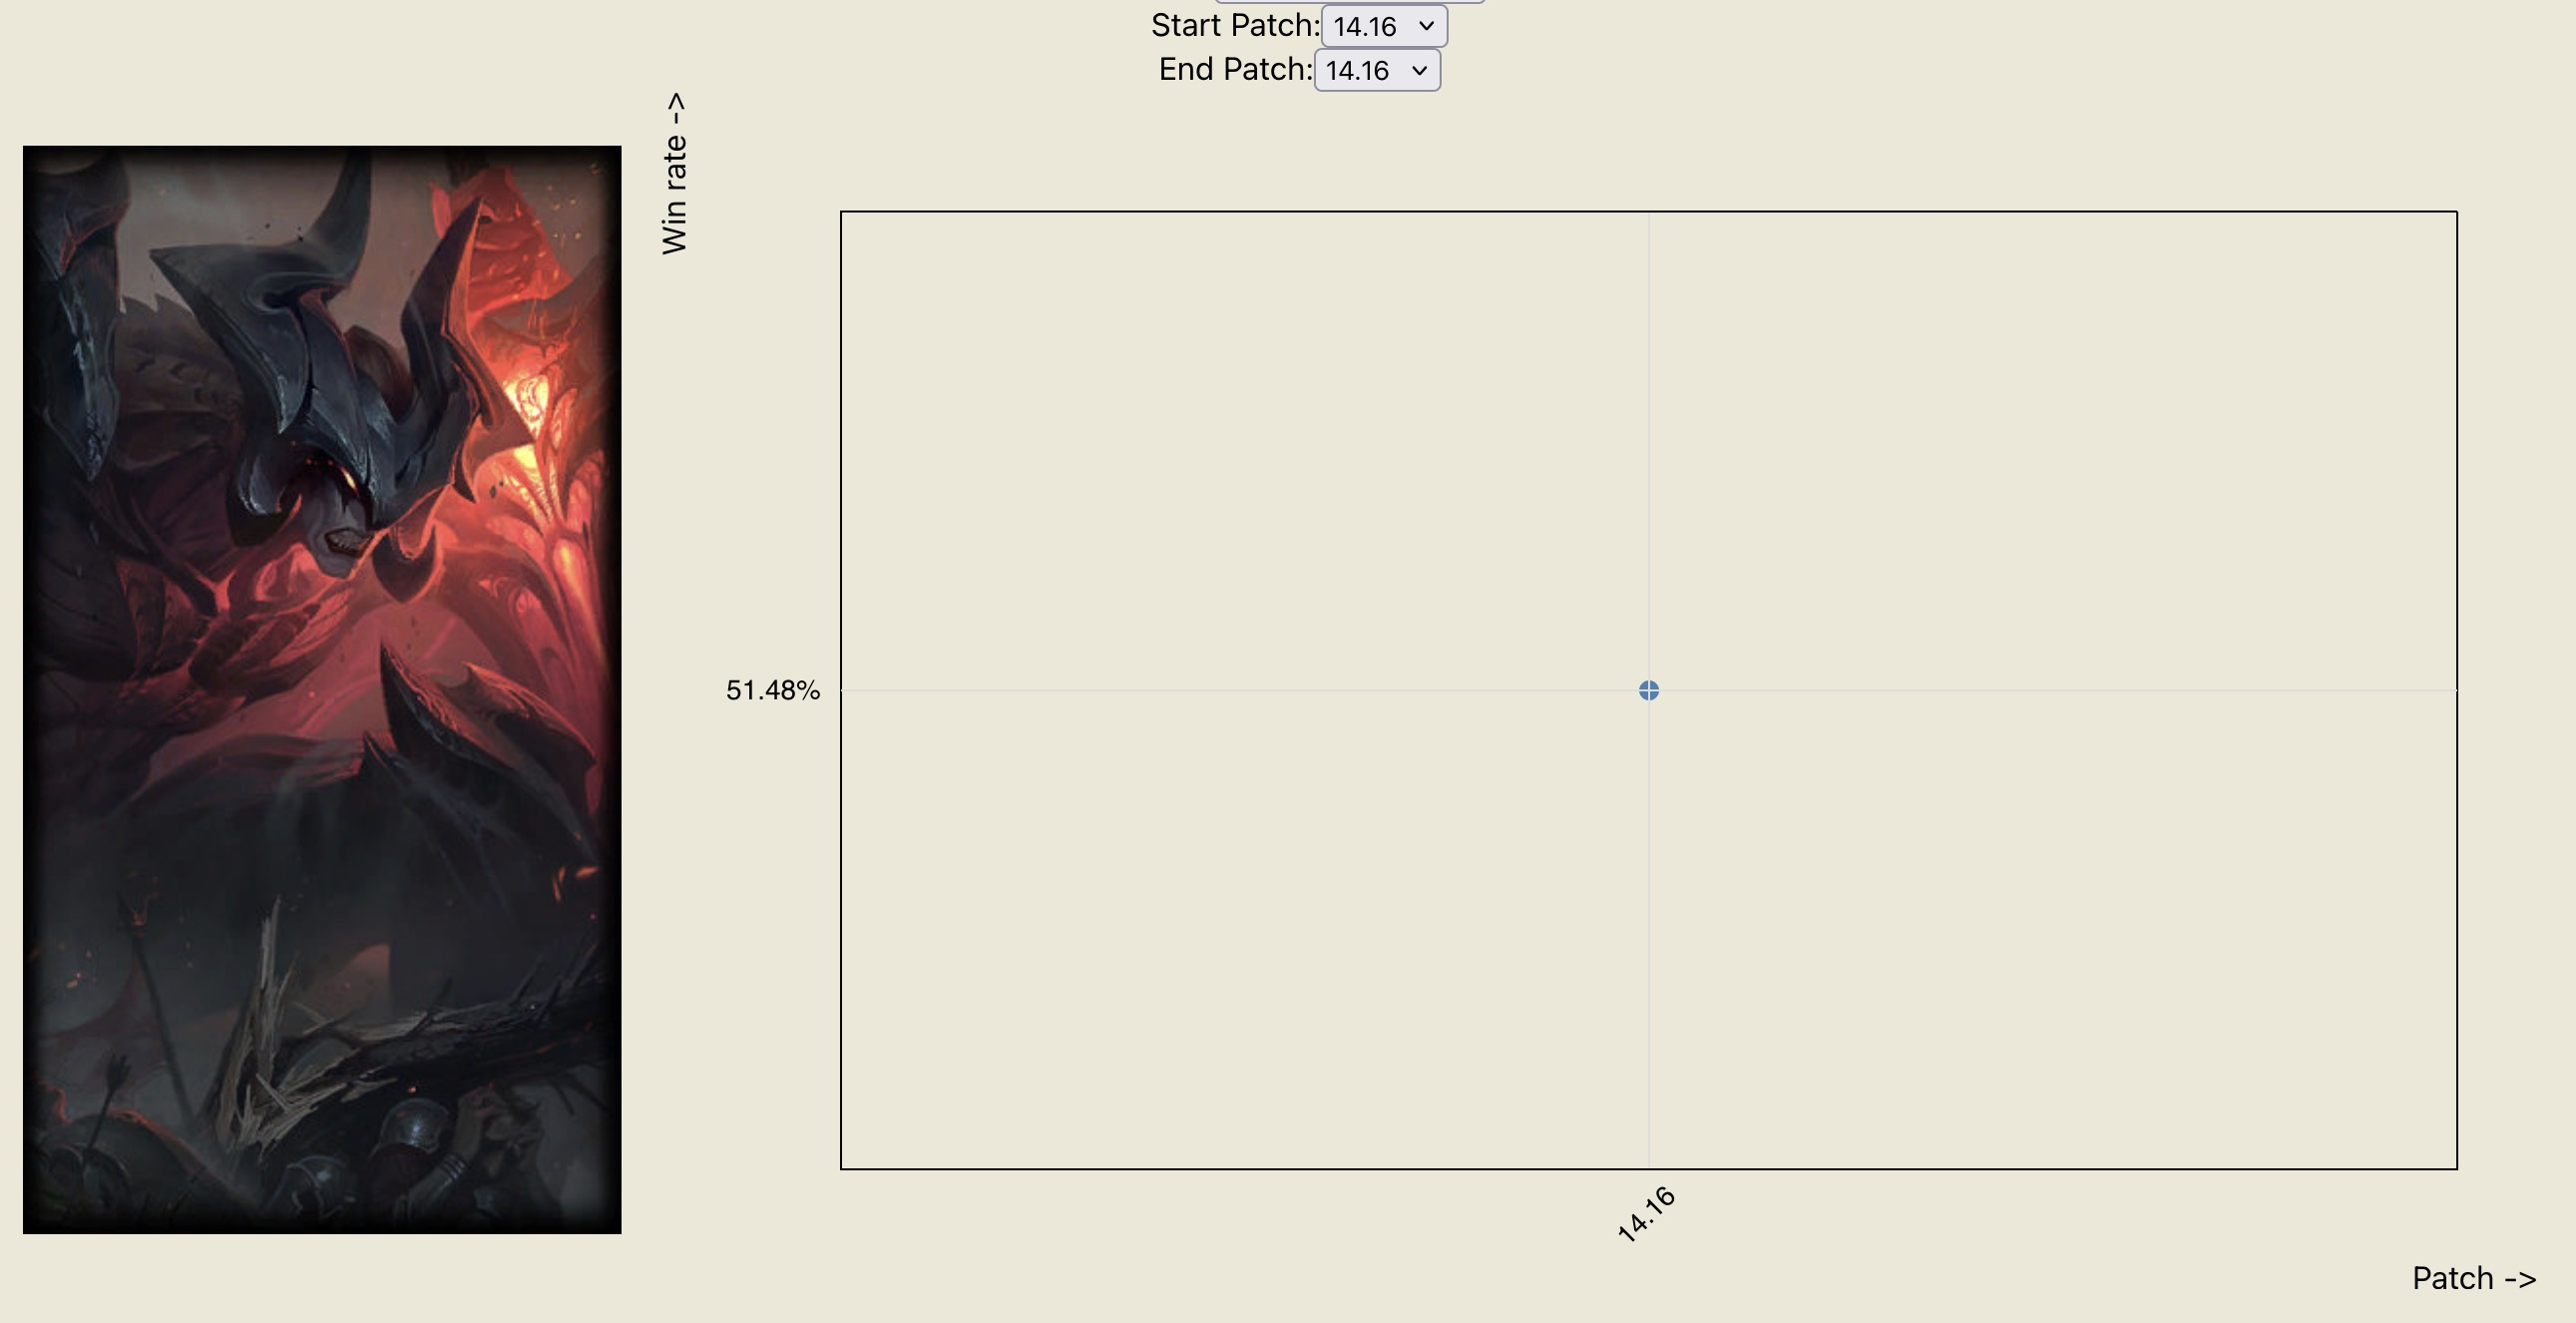
\includegraphics[width=0.75\textwidth]{figs/one.jpg}
  \caption{
      Solo patch range.
  }
  \label{fig:fig2}
\end{figure}

\begin{figure}[ht] 
  \centering
  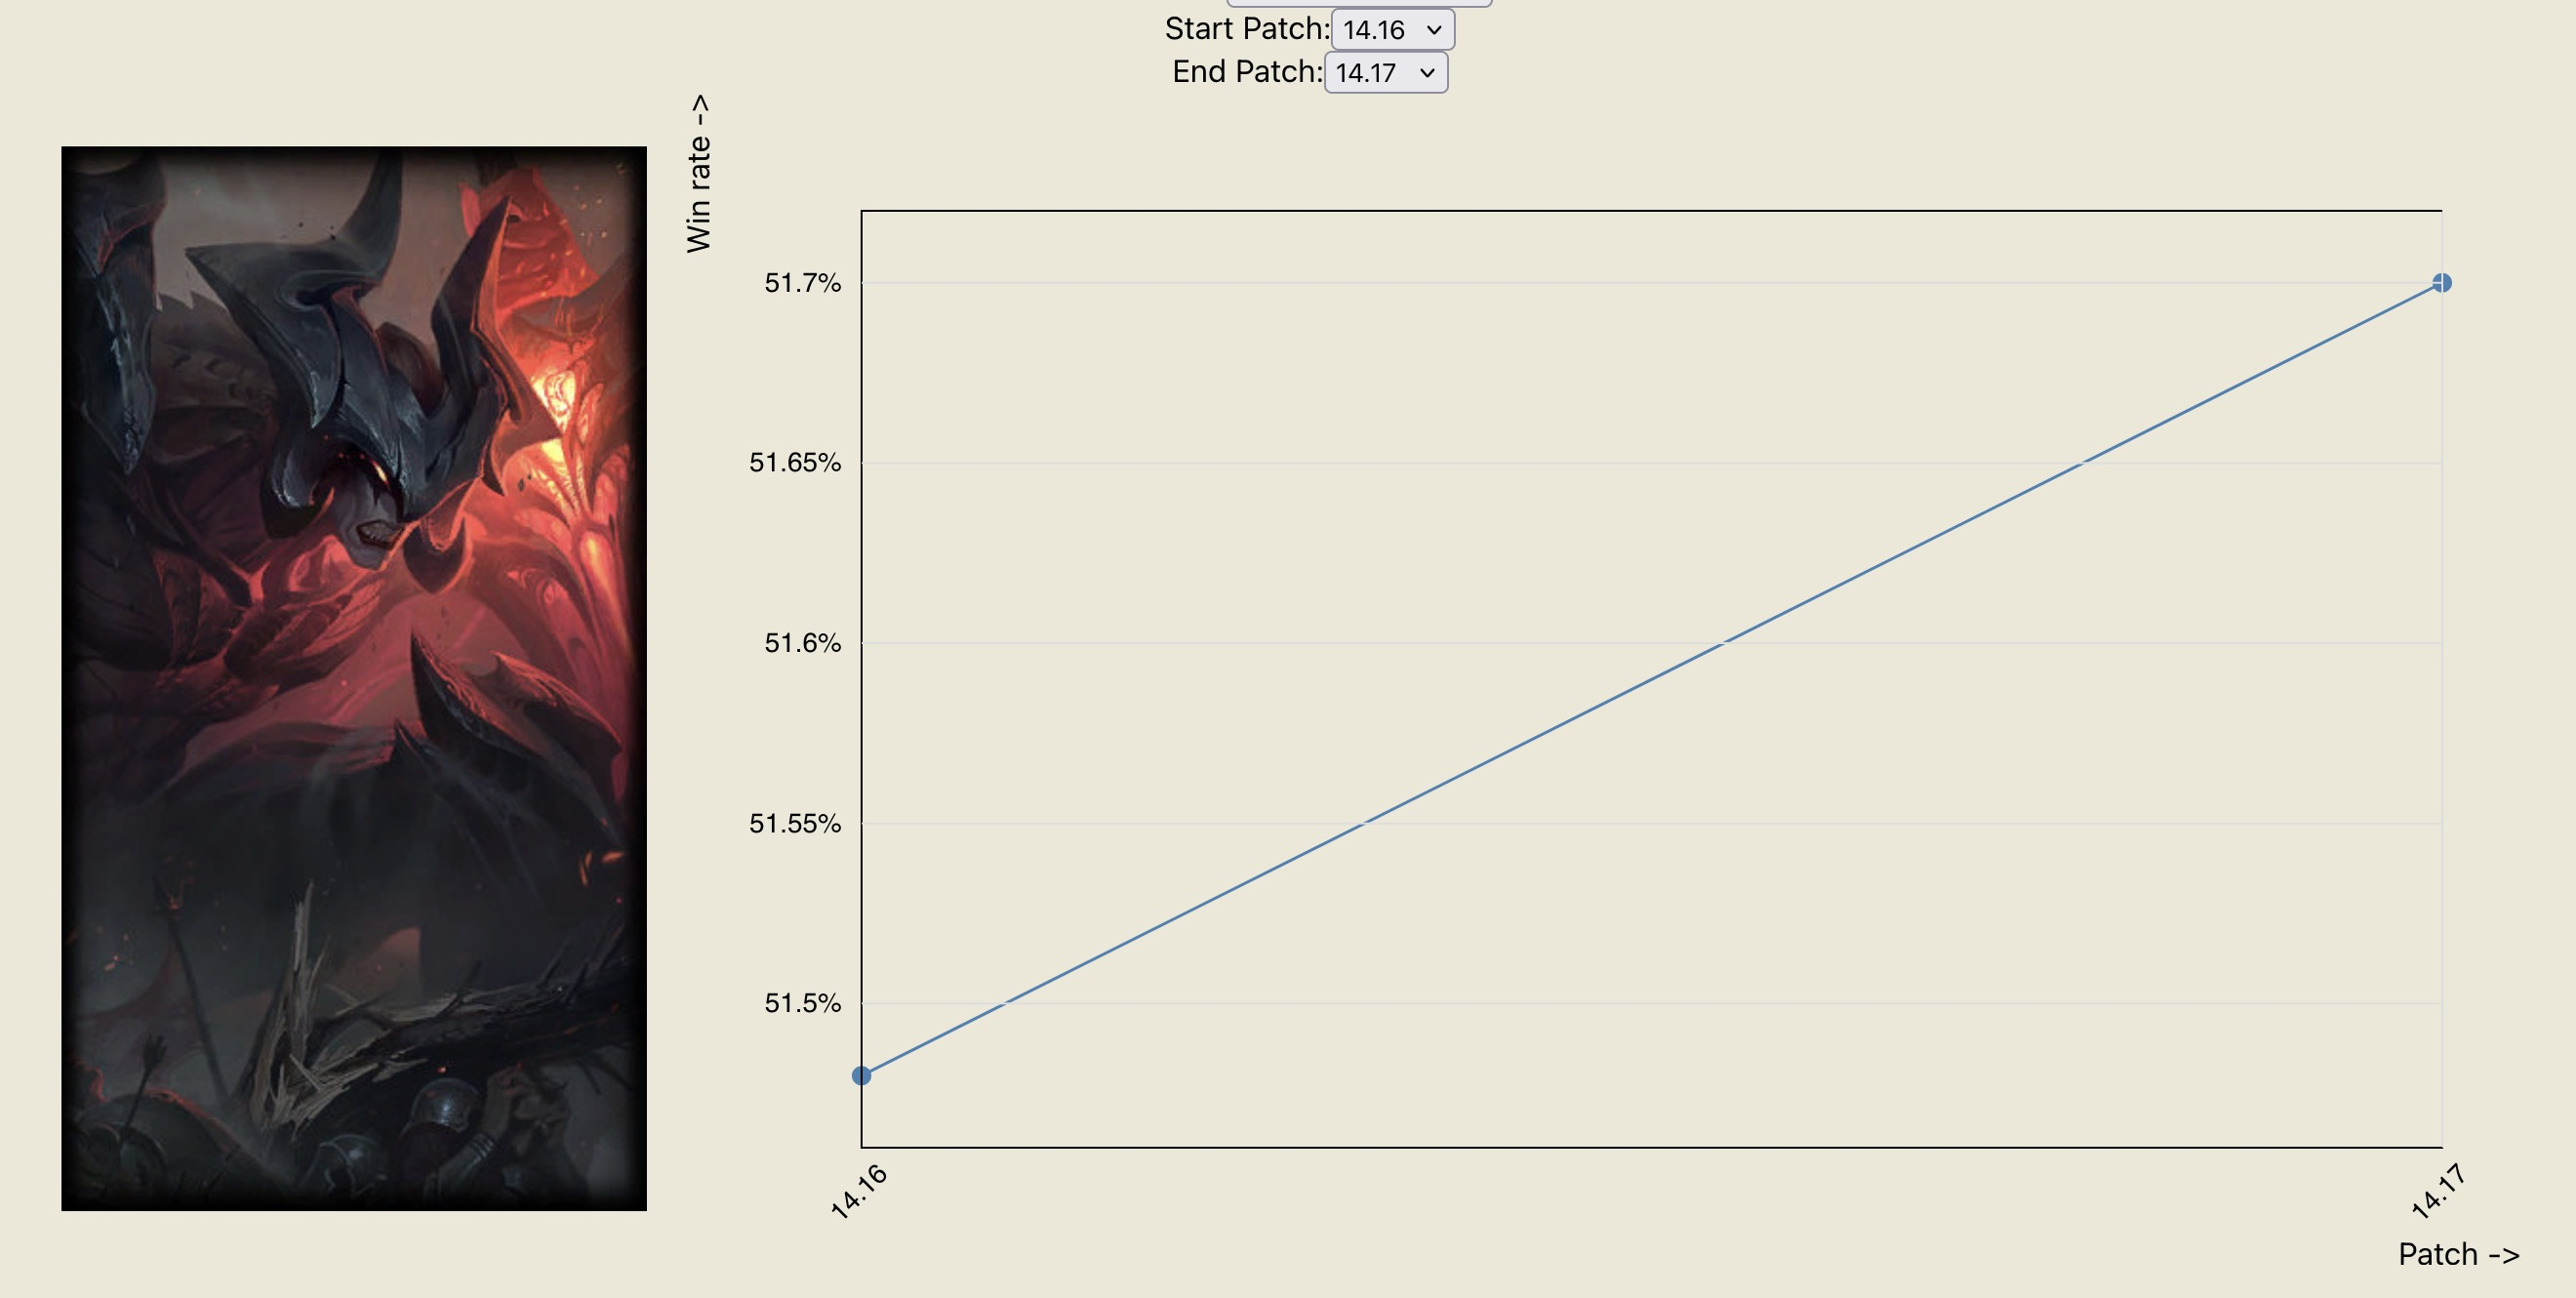
\includegraphics[width=0.75\textwidth]{figs/two.jpg}
  \caption{
      Size 2 patch range.
  }
  \label{fig:fig3}
\end{figure}

I did not create a fix for this specific situation, since the Visualization is 
for users to see how their champion has been impacted over time.

\subsubsection{Lane Specific Data}
\label{subsubsec:Lane Specific Data}

Another piece of feedback was to include lane specific data.

Why? Well, a botlane champion will have a different winrate if they are played toplane. 
In layman's terms, the best pizza is not a very good burger. 
Also, some champions are played in multiple lanes, so it would be interesting to see
how their winrate changes depending on the lane.

I deemed this to be beyond the scope of the assignment, but it is a good idea.

\subsection{Conclusion: Do we answer the question?}
\label{subsec:Conclusion}

I believe for both:

\begin{enumerate}
  \item How has my champion's win rate changed over time?
  \item Is my champion still strong in the current meta?
\end{enumerate}

We more than answer the question. By providing additional data like rank,
winrate delta, and games, we allow the user to make a more informed decision
on whether their champion is strong or not.

Corki was just buffed on Wednesday (and I hate that), do these images answer both questions? 

\begin{figure}[ht] 
  \centering
  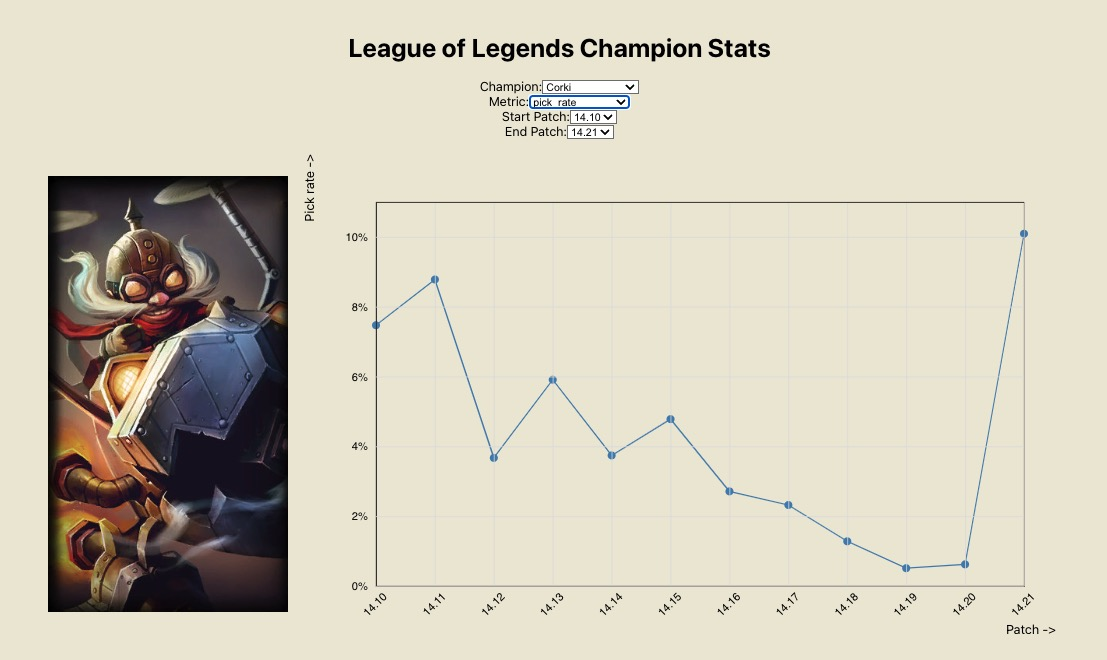
\includegraphics[width=0.75\textwidth]{figs/corki1.jpg}
  \caption{
      Corki Pick Rate
  }
\end{figure}

\begin{figure}[ht] 
  \centering
  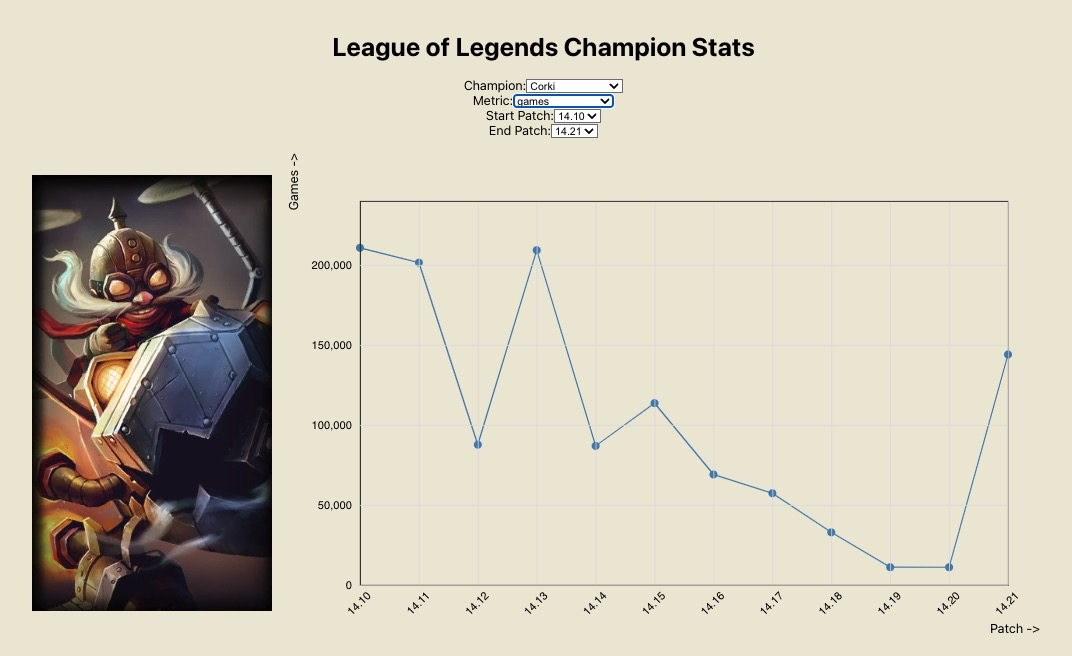
\includegraphics[width=0.75\textwidth]{figs/corki2.jpg}
  \caption{
      Corki Games Played
  }
\end{figure}

\begin{figure}[ht] 
  \centering
  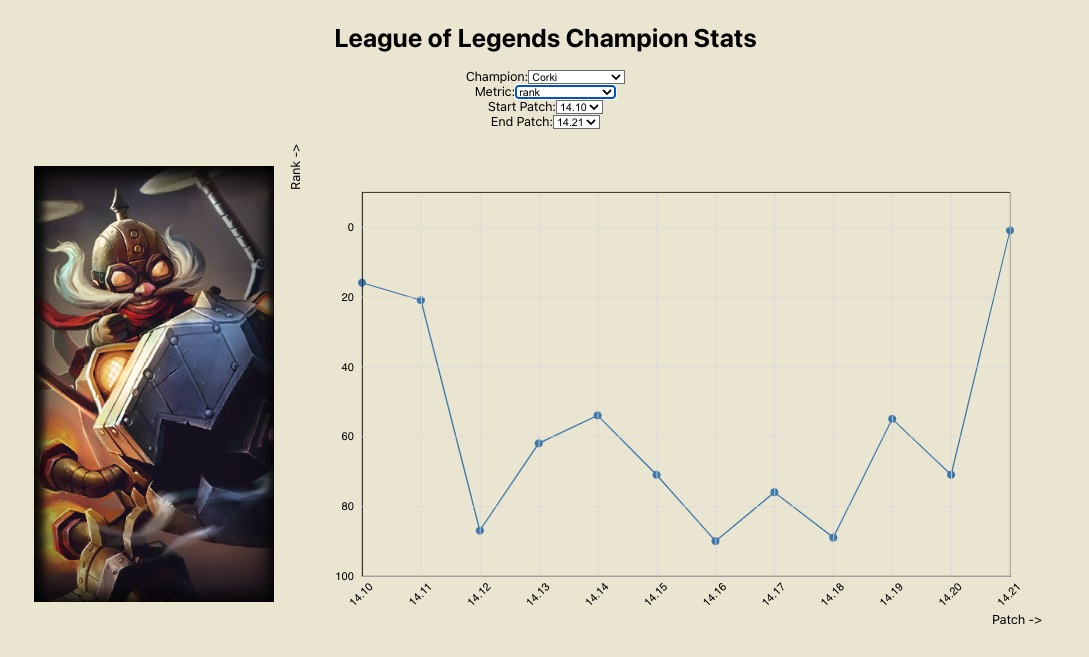
\includegraphics[width=0.75\textwidth]{figs/corki3.jpg}
  \caption{
      Corki Rank
  }
  \label{fig:fig3}
\end{figure}

\begin{figure}[ht] 
  \centering
  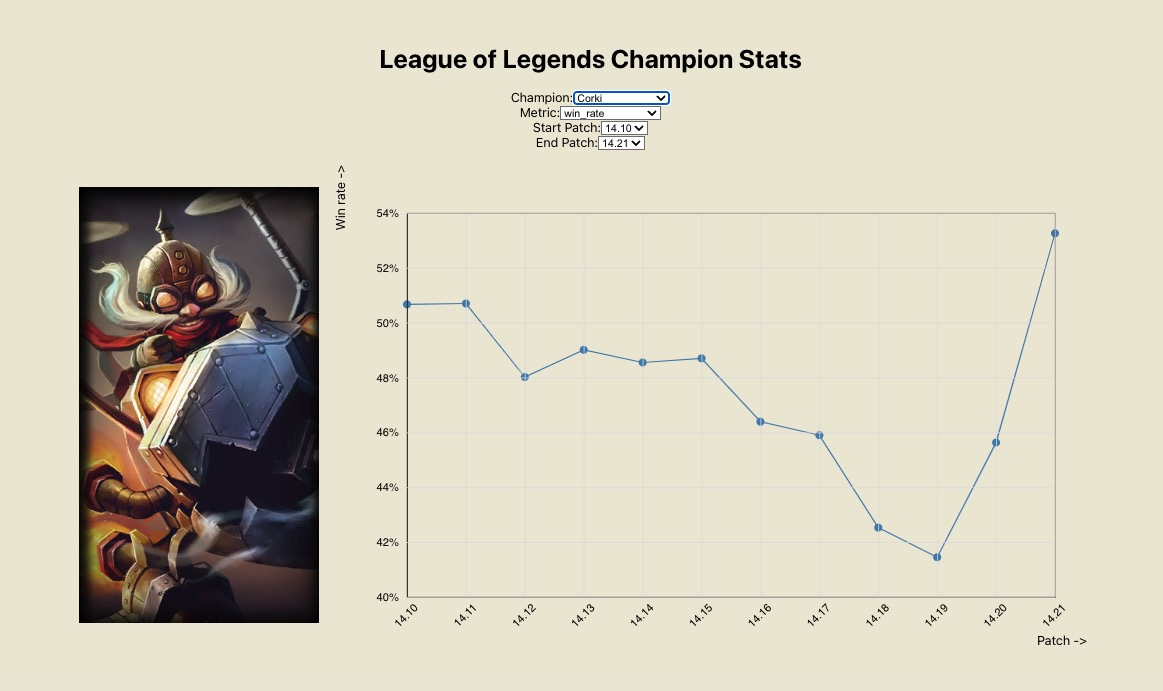
\includegraphics[width=0.75\textwidth]{figs/corki4.jpg}
  \caption{
      Corki Winrate
  }
  \label{fig:fig3}
\end{figure}

\begin{refcontext}[sorting=nyt]
\printbibliography
\end{refcontext}

\end{document}

